\documentclass[a4paper, 11pt]{article}
\usepackage{comment}
\usepackage{fullpage}
\usepackage{blindtext}
\usepackage{graphicx}
\usepackage{listings}
\usepackage{color}
\graphicspath{ {./images/} }

\definecolor{dkgreen}{rgb}{0,0.6,0}
\definecolor{gray}{rgb}{0.5,0.5,0.5}
\definecolor{mauve}{rgb}{0.58,0,0.82}

\lstset{frame=tb,
  language=Java,
  aboveskip=3mm,
  belowskip=3mm,
  showstringspaces=false,
  columns=flexible,
  basicstyle={\small\ttfamily},
  numbers=none,
  numberstyle=\tiny\color{gray},
  keywordstyle=\color{blue},
  commentstyle=\color{dkgreen},
  stringstyle=\color{mauve},
  breaklines=true,
  breakatwhitespace=true,
  tabsize=3
}

\begin{document}

\title{Computer Science 221: Design Patterns and OOP}

    \maketitle

\section{Introduction}

    The following goes over information pertinent to material taught both in-class and out-of-class.

    The material covered on exam 1 include:

    \begin{itemize}
        \item Imperative vs Object-oreinted style
        \item UML
        \item Singleton Design Pattern
        \item Abstraction
        \item Debugger
        \item Polymorphism
        \item Dispatch/Double Dispatch
        \item Interfaces, arrays, lists
        \item Generics
        \item Enhanced For Loops
        \item Casting
        \item Exception Handling
        \item Java Virtual Machine
        \item Observer Design Pattern
    \end{itemize}

    The material convered on exam 2 include:

    \begin{itemize}
        \item State Design Pattern
        \item Requirements Gathering
        \item MVC
        \item Static Initializers
        \item Declarative Style
        \item java.lang.Map
        \item Abstraction Violation
        \item Java Streams
        \item Downcasting (Reprise)
        \item Git
        \item Debugger
        \item Strategy Design Pattern
        \item Java Swing
        \item Java Listeners
        \item SOAP and RESTFUL
        \item Jersey (RESTFUL)
    \end{itemize}

\newpage

\section{Notation}
    \subsection{UML}
        UML (Unified Modeling Language) is a standard language for visualizing and documenting software systems.
        \begin{center}
            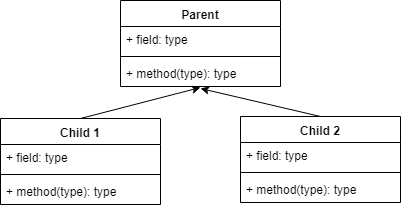
\includegraphics[scale=0.8]{uml_basic}
        \end{center}
        The following image depcits the meaning of arrow association:
        \begin{center}
            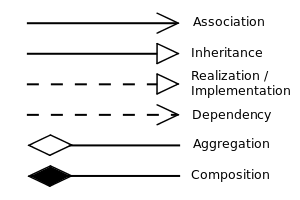
\includegraphics{uml_arrow}
        \end{center}
        The following image depcits the meaning of classes structure:
        \begin{center}
            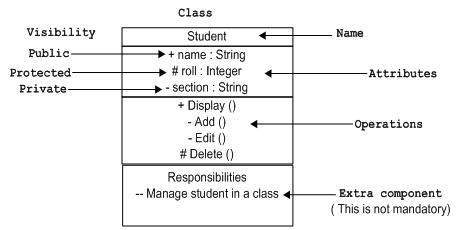
\includegraphics[scale=0.8]{uml_class}
        \end{center}

\section{OOP Concepts and Introduction}

    \subsection{Imperative State vs. Object Oriented Design}
        An imperative style is a procedural method for programming that goes through a list of procedures modifying the state of variables through a sequence of testing states (If statements).
        \newline\newline
        An Object Oriented Design is a structure for storing objects, a data structure holding state and behavior.  An object-based language is one that has objects while an object-oriented language is an object-based language with inheritance.

    \subsection{Classes}
        A class is a blueprint with:
        \begin{itemize}
            \item Fields (Instance Variables): What an object knows
            \item Methdos (Functions): What an object does
        \end{itemize}

    \subsection{Inheritance}
        What do classes have in common?  Classes have features abstracted from a parented class.  Methods can be overrided or extended that don't work.
        \newline\newline
        Class inherit from a super class in order to define fields and methods defined in the super class.
        \newline\newline
        To decide on what inherits what, follow the rules:
        \begin{itemize}
            \item "Is A" helps decide if a class should extend another\\
                i.e. Is a dog an "Animal"
            \item "Has A" helps decide if something is a field\\
                i.e. "Dog" has a "Height"
        \end{itemize}
        \textbf{Do not use inheritance purely to reuse code, especially if it does not follow the rules}
        \newline\newline
        Why use inheritance?
        \begin{itemize}
            \item Reduces code
            \item Reduces duplicate code
            \item Changes to parent classes are inherited by children
        \end{itemize}

    \subsection{Encapsulation}
        Allows certain classes to only be accessible by certain types.  This is defined by the following:
        \begin{itemize}
            \item Public: Any class can access
            \item Protected: Only child classes can access
            \item Private: Only the class can access the object
        \end{itemize}

    \subsection{Abstraction}
        Allows you to define an outline of how each class that inherits from an abstract class should be structured.  This provides the power of Polymorphism without the work.  There are no abstract fields.  All the methods do not have to be extract.
        \newline\newline
        Abstraction allows you to handle complexity by hiding unnessary details from the user, enabling the user to implemnt more complex logic on top of already complex logic, defined by the abstraction without understanding the hidden complexity within the abstraction.
        \newline\newline
        A real world example is making coffee.  You, the user, only needs to know the logic on how to operate the coffee machine.  You do not need to know how the coffee machine works to get a good result.
        \newline\newline
        An abstract base class (ABC) corresponds to an abstract concept instead of an object.  For example, a "Vehicle" is more of an idea than an object since there are many kinds of vehicles.  Therefore a vehicle would be an abstract base class whereas a "Car" is more suited to be a regular abstract class since a car is much more of a concrete idea than a vehicle.
        \newline\newline
        In Java, abstract classes and methods can be defined by adding the "abstract" keyword.  Note that any object with an abstract method is considered to be abstract.  Note that a class needs to be abstact to have abstract methods.  This just means that only subclasses that implement that method can call it.

    \subsection{Polymorphism}
        Polymorphism describes situations in which something occurs in several different forms.  More specificaly in OOP, it describes the concept that objects of differnt types can be accessed thorugh the same interface, each providing its own independent implementation of a interface.
        \newline\newline
        Polymorphism allows you to write methods that don't need to change if new subclasses are created.
        For example, an object can add method without affecting the parent class and an object can override a method without affecting the parent.  As a result, you can refer to differnt subclasses based on the parent class.
        \newline\newline
        Note that you \textbf{cannot} call classes for subclasses.  For example, if you have an animal, Dog (refered to as type animal), you cannot make it bark unless you cast it.
        \newline\newline
        There are 2 types of Polymorphism:
        \begin{itemize}
            \item Parametric polymorphism: Allows a single piece of code to be typed generically, using variables instead of actual types, which are instantiated to particular types when needed.
            \item Ad-hoc polymorphism: Allows polymorphic value to exhibit differnt behaviors when "viewed" at different types.  Usually, this comes in the form on overloading, which associates a single function sybmol with many implementations.  The compiler or runtime system, depending if it is static or dynamic, will choose the appropriate implementation for each function based on the arguments.
        \end{itemize}
        \begin{center}
            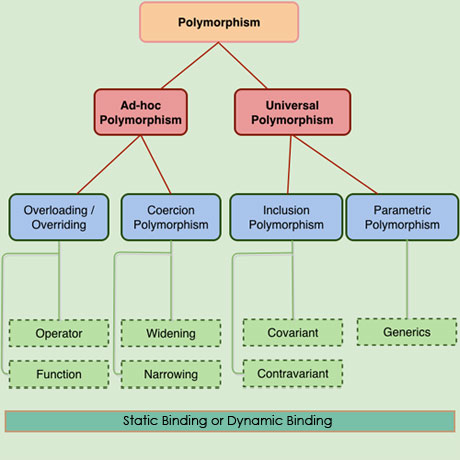
\includegraphics[scale=0.8]{polymorphism}
        \end{center}

    \subsection{Dispatch}
        Dipatch is the mechanism by which an overriden method is resolved at run-time instead of compile time.  Note that overridden methods usually are a result of polymorphism (Overloading occurs when two or more methods have the same method name but different parameters and ovverriding means having two or more methods with the same method name and parameters, but different implementation thoughtout different classes).
        \newline\newline
        When overriden methods are called, Java determines which class (super/subclass) of that method to execute based upon the type of the object being called.  Doing so allows:
        \begin{itemize}
            \item Java to support overriden methdos which is essential for run-time polymorphism
            \item A class to specify methods that will be common to all of its derivatives (Descendents) while allowing subclasses to define specific implementation of some of those methods
            \item Subclasses to add its spec methods to subclasses to detefine the specific implementation of some.
        \end{itemize}
        Double dispatch is a methods to allow dynamic binding (Single dispatch) alongside overloading methods.
        \newline\newline
        Double dispatch is a special form of multiple dispatch, and a mechanism that dispatches a function call to different concrete functions depending on the runtime types of two objects involved in the call. In a mxn matrix, the first dispatch will run on row, and the second dispatch will run on column to determine the correct method to run.

    \subsection{Interfaces}
        \begin{itemize}
            \item a class with only abstract Methods
            \item Add as many interfaces to implement
            \item only use public static and final Fields
        \end{itemize}
        A class with only abstract methods.

    \subsection{Casting}
        Casting object in OOP is usually the product of eith class inheritance or interface inheritance.   Class inheritance denotes an “is a” relationship whereas an interface inheritance denotes an “has a” relationship.
        \newline\newline
        Upcasting is casting a subtype to a supertype, upward to the inheritance tree. Upcasting happens automatically and we don’t have to explicitly do anything.

    \subsection{Declarative Style}
        When using method with one-liners. Non-imperative style of programming; keeps code in the domain as long as possible and makes the code more readable.

    \subsection{Array Interface Contradiction}
        Something to do with the types arrays and lists can hold so switching between the two would cause problems if a list were to become an array of types it cannot hold.

    \subsection{Requirements Gathering}
        The idea of bouncing ideas between peers in order to determine the optimal approach for solving a problem.  For example, creating a list of ideas for requirements.

    \subsection{Abstraction Violation}
        Occurs when an object’s abstraction barrier (definitions for abstraction) is violated, such that its data is accessed directly when the object, itself, is in use.  This means that the field itself is being accessed instead of using a “getter” method.  Violating abstraction usually results in having a single object calling various of its subfields :
        \begin{lstlisting}
        (list.stream().map(Item::getName).collect(Collectors.joining(", ")));
        \end{lstlisting}

    \subsection{Model View Controller (MVC)}
        Architecture/design, useful for GUI, web design, which allows for efficient code reuse and parallel development (we can reuse methods with ease, and people can be working on model, while others are working on view, and others on controller)
        \begin{itemize}
            \item \textbf{M}odel: The backend of the project - Defines the essential components representing, usually, the real-world aspects of the application.
            \item \textbf{V}iew: The frontend of the project - Functions that the user actually interact with the user, usually through a GUI (graphical user interface).
            \item \textbf{C}ontroller: The interfacing aspect that interfaces between the model and view
        \end{itemize}

\newpage

\section{JAVA}

    \subsection{Arrays}
        An array is a group of like-typed variables that are referred to by a common name.
        \begin{itemize}
            \item In Java all arrays are dynamically allocated.
            \item Since arrays are objects in Java, we can find their length using member length.
            \item A Java array variable can also be declared like other variables with [] after the data type.
            \item The variables in the array are ordered and each have an index beginning from 0.
            \item Java array can be also be used as a static field, a local variable or a method parameter.
            \item The size of an array must be specified by an int value and not long or short.
            \item The direct superclass of an array type is Object.
            \item Every array type implements the interfaces Cloneable and java.io.Serializable.
        \end{itemize}
        Array can contains primitives data types as well as objects of a class depending on the definition of array. In case of primitives data types, the actual values are stored in contiguous memory locations. In case of objects of a class, the actual objects are stored in heap segment.

    \subsection{Lists}
        The Java.util.List is a child interface of Collection. It is an ordered collection of objects in which duplicate values can be stored. Since List preserves the insertion order, it allows positional access and insertion of elements. List Interface is implemented by ArrayList, LinkedList, Vector and Stack classes.

    \subsection{Generics}
        Generics in Java allow type to be a paramter to a method and interfaces.  Doing so allows the user to define different tyoes of a method, class, and interface.  Generics provide the benefits:
        \begin{itemize}
            \item Code Reduction: Write a method/class/interface once for any type desired
            \item Type Safety: Generics make errors to appear compile time rather than at run time.
        \end{itemize}

    \subsection{Exception Handling}
        Whenever an error occurs while executing a statement, creates an exception object and then the normal flow of the program halts and JRE tries to find someone that can handle the raised exception.

    \subsection{Java Virtual Machine}
        A Java virtual machine (JVM) is a virtual machine that enables a computer to run Java programs as well as programs written in other languages and compiled to Java bytecode. The JVM is detailed by a specification that formally describes what is required of a JVM implementation.
        \newline\newline
        During compile time, the JVM runs 1. source code (.java) 2. Compiler (Object in .class) 3. Java.exe or java (java using -cp [class path])
        \newline\newline
        Difference between JVM and C++ compiler 1.) Object and library through a Linked. 2.) Executable
        \newline\newline
        Physical System:
        \begin{itemize}
            \item CPU
            \item Arithmetic Logical Unit (ALU)
            \item Memory System
            \item Physical Machine
        \end{itemize}

    \subsection{Reflection}

    \subsection{Casting}

    \subsection{Debugger}
        Set a \textbf{breakpoint} which stops execution and allows for:
        \begin{itemize}
            \item Resume: continue until the next breakpoint
            \item Step: move to the next line after executing the current line
            \item Step into: steps through method invocations on the current line. (e.g. it may go to the first line of a method somewhere else that is called.)
            \item Step out:  executes the rest of the current method and stops execution at the line from which the current method was called.
        \end{itemize}
        Set a \textbf{watchpoint} to stop execution when a specified variable changes value.

    \subsection{java.lang.Map}
        \begin{lstlisting}
        public interface Map<K,V>
        \end{lstlisting}
        An object that maps keys to values. A map cannot contain duplicate keys; each key can map to at most one value. The Map interface provides three collection views, which allow a map's contents to be viewed as a set of keys, collection of values, or set of key-value mappings. The order of a map is defined as the order in which the iterators on the map's collection views return their elements. Some map implementations, like the TreeMap class, make specific guarantees as to their order; others, like the HashMap class, do not.

    \subsection{Java Stream}
        A stream is a sequence of objects that supports various methods which can be pipelined to produce the desired result.  The features of Java stream are:
        \begin{itemize}
            \item A stream is not a data structure instead it takes input from the Collections, Arrays or I/O channels.
            \item Streams don’t change the original data structure, they only provide the result as per the pipelined methods.
            \item Each intermediate operation is lazily executed and returns a stream as a result, hence various intermediate operations can be pipelined. Terminal operations mark the end of the stream and return the result.
        \end{itemize}
        Some intermediate operations include the following:
        \begin{enumerate}
            \item \textbf{map}: The map method is used to map the items in the collection to other objects according to the Predicate passed as argument.
            \begin{lstlisting}
            List number = Arrays.asList(2,3,4,5);
            List square = number.stream().map(x->x*x).collect(Collectors.toList());
            \end{lstlisting}
            \item \textbf{filter}: The filter method is used to select elements as per the Predicate passed as argument.
            \begin{lstlisting}
            List names = Arrays.asList("Reflection","Collection","Stream");
            List result = names.stream().filter(s->s.startsWith("S")).collect(Collectors.toList());
            \end{lstlisting}
            \item \textbf{sorted}: The sorted method is used to sort the stream.
            \begin{lstlisting}
            List names = Arrays.asList("Reflection","Collection","Stream");
            List result = names.stream().sorted().collect(Collectors.toList());
            \end{lstlisting}
        \end{enumerate}

    \subsection{Java Swing}
        Swing is a GUI widget toolkit for Java.[1] It is part of Oracle's Java Foundation Classes (JFC) – an API for providing a graphical user interface (GUI) for Java programs.
        \begin{center}
            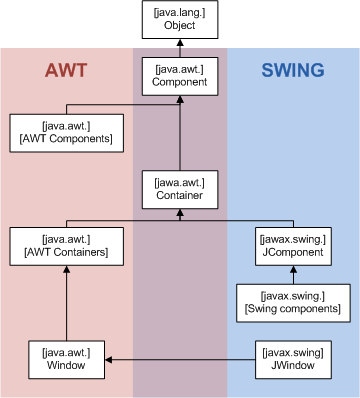
\includegraphics[scale=0.8]{swing}
        \end{center}
        \begin{itemize}
            \item AWT - Abstract widget toolkit - inside default GUI for Java
            \item Swing - better GUI, not default
            \item JFrame - Creates the frame with dimensions to create applications in it.
            \item Jpanel - Container for widgets (Constructor)
            \item JBorderLayoutManager - creates the border of and in which cardinals directions and center are defined.
        \end{itemize}

    \subsection{SOAP and RESTful}
        SOAP and RESTful are two popular styles of webs services, SOAP using XML formatting while RESTful uses the HTTP protocol.\\
        SOAP:
        \begin{itemize}
            \item Simple Object Access Protocol (Old Name)
            \item Service Oriented Architecture Protocol (More current Name)
        \end{itemize}
        SOAP stands for Simple Object Access Protocol. It’s a messaging protocol for interchanging data in a decentralized and distributed environment. SOAP can work with any application layer protocol, such as HTTP, SMTP, TCP, or UDP. It returns data to the receiver in XML format. Security, authorization, and error-handling are built into the protocol and, unlike REST, it doesn’t assume direct point-to-point communication. Therefore it performs well in a distributed enterprise environment.\\
        RESTful:
        \begin{itemize}
            \item Representational State Transfer
        \end{itemize}
        The RESTful API is used more by the community since it uses a Uniform Resourece Identifer (URI) and  implements the HTTP transport protocol defined by Roy Fielding's PHD Thesis.  His thesis's abstract is as follows:
        \newpage\newpage
        \textit{The Hypertext Transfer Protocol (HTTP) has a special role in the Web architecture as both the primary application-level protocol for communication between Web components and the only protocol designed specifically for the transfer of resource representations. Unlike URI, there were a large number of changes needed in order for HTTP to support the modern Web architecture. The developers of HTTP implementations have been conservative in their adoption of proposed enhancements, and thus extensions needed to be proven and subjected to standards review before they could be deployed. REST was used to identify problems with the existing HTTP implementations, specify an interoperable subset of that protocol as HTTP/1.0 [19], analyze proposed extensions for HTTP/1.1 [42], and provide motivating rationale for deploying HTTP/1.1. The key problem areas in HTTP that were identified by REST included planning for the deployment of new protocol versions, separating message parsing from HTTP semantics and the underlying transport layer (TCP), distinguishing between authoritative and non-authoritative responses, fine-grained control of caching, and various aspects of 117 the protocol that failed to be self-descriptive. REST has also been used to model the performance of Web applications based on HTTP and anticipate the impact of such extensions as persistent connections and content negotiation. Finally, REST has been used to limit the scope of standardized HTTP extensions to those that fit within the architectural model, rather than allowing the applications that misuse HTTP to equally influence the standard.}
        \newpage\newpage
        The REST guidelines allow developers to implement the details according to their own needs. Web services built following the REST architectural style are called RESTful web services.  We can specify the HTTP commands \textbf{GET, PUT, POST, DELETE} by using the @ commands. For example @Path("/helloWorld") gives the tail end of the path for the URI and @GET comes before the meothods definition for what verbs has to happen for the method to be called and @Produces(MediaType.someTypeOfText) to declare the produce type - plain, XML, etc.  To create a REST API, you need to follow six architectural constraints:
        \begin{itemize}
            \item Uniform interface – Requests from different clients should look the same, for example, the same resource shouldn’t have more than one URI.
            \item Client-server separation – The client and the server should act independently. They should interact with each other only through requests and responses.
            \item Statelessness – There shouldn’t be any server-side sessions. Each request should contain all the information the server needs to know.
            \item Cacheable resources – Server responses should contain information about whether the data they send is cacheable or not. Cacheable resources should arrive with a version number so that the client can avoid requesting the same data more than once.
            \item Layered system – There might be several layers of servers between the client and the server that returns the response. This shouldn’t affect either the request or the response.
            \item Code on demand [optional] – When it’s necessary, the response can contain executable code (e.g. JavaScript within an HTML response) that the client can execute.
        \end{itemize}
        In class, we used specific implementations of RESTful: Jersey and Grizzly.

        \subsubsection{Jersey and Grizzly}
            Simplifies development of RESTful Web services and their clients in Java.  This framework is open source (via Github) and provides an API that extends JAX-RS toolkit (Java Restful implementation - not in scope of course).  Usually, the Grizzly Web server is used for the web server component for the application by offering an easy scalable and robust servers and extended frameworks such as the web framework (HTTP/S).

    \subsection{Static Initializers}
        Initializer blocks to initialize instance variables.  The blocks are not executed until the class instance is created therefore disallowing access before the class is created.  A static initializer can be used to create static fields and access them before the class is created (created at initialization).

        \begin{lstlisting}
            static {
            	Statements…
            }
        \end{lstlisting}

\newpage

\section{Design Patterns}

    \subsection{Strategy}
        Encapsulation of related interchangeable algorithms such that they are independent from the clients that use them.  Essentially, multiple algorithms are defined in classes for unique, but related, strategies.  The game developed in class implements this strategy by having different objects based on their specific needs (for example there are multiple inventory systems depending on what the context is - which inventory system the player wants - or the direction since the CompassDirection represents a specific strategy for the direction).  This reduces the complexity of the client-context object since they do not need each individual algorithm that they could possibly need to be implemented, further reducing the number of if-statements and making future related algorithms to be easier to implement, as in homework 3.
        \begin{center}
            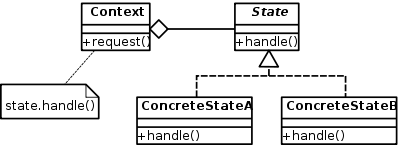
\includegraphics[scale=0.8]{state}
        \end{center}
        The three participants of this include:
        \begin{itemize}
            \item Context: Defines the status of the program the determines which strategy should be implemented.
            \item Strategy: The strategy of an object (interface for concrete strategy to inherit from).
            \item ConcreteStrategy: The possibele strategyies for the object.
        \end{itemize}

    \subsection{Observer}
        Defines a one-to-many dependancy between objects such that the state of all dependant objects relies on the state of a single object by being notified such that they are updated automatically.  By reducing the direct relationship between the state of each objects (such that one object will consistently directly update the other) the objects become much more reusable.  This is most predominant in graphical user interfaces (GUIs).  In a GUI, a panel, the \textbf{subject/publisher}, will \textbf{notify} by basically sending a signal.  Any \textbf{observers/subscribers} who recieve this signal will then act based on this signal.
        \begin{center}
            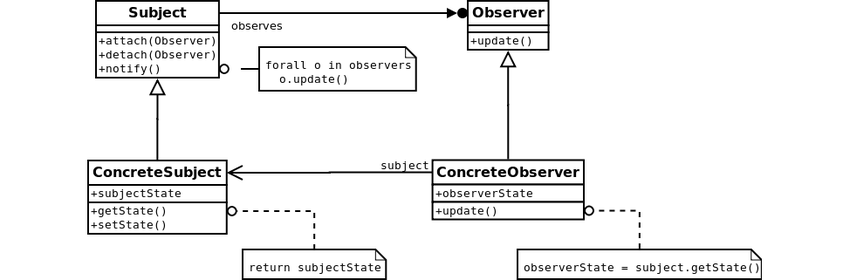
\includegraphics[scale=0.6]{observer}
        \end{center}
        The three particapants are:
        \begin{itemize}
            \item Subject: An interface for objects to implement in order to define what to notify actions to
            \item Observer: An updating interface for objects that should be notified of changes in the subject
            \item ConcreteSubject: The object that we are observing and of interest (we want other objects to act based on the subject's actions)
            \item ConcreteObserver: The object that should be updated whenever the subject's state is changed.
        \end{itemize}
        In GUI, Event listeners represent the interfaces responsible to handle events. Java provides various Event listener classes, however, only those which are more frequently used will be discussed. Every method of an event listener method has a single argument as an object which is the subclass of EventObject class. For example, mouse event listener methods will accept instance of MouseEvent, where MouseEvent derives from EventObject.

    \subsection{Factory}

    \subsection{Abstract Factory}

    \subsection{Singleton}
        The singleton pattern is a design pattern that restircts the instatiation of a class to one object.
        \newline\newline
        Singletons are used when you want to eliminate the option instantiating more than one object.  An example of when to use this is using a class to hold all the potential scrabble letter and spits out new ones upon request.
        \begin{itemize}
            \item Lazy (Classic) instantiation: If the instance is never needed, it will never be created.  The main problem is taht the the thread is not safe since two threads can attempt to create Singletons at the same time causing 2 singletons to be created, making the idea of a singleton to be violated.
            \item Eager instatiation: Creates an instance of singletoon in the static initializer.  The JVM executes the static initializer when the class is laded ang guarantees the thread to be safe.  This should only be used when the singleton class is loight and is used thoughpout the execution of your program.
            \item Synchronizing instantiation: Using the sychornized makes sure that only one thread can refer (call the getInstace method) at once.  The issue is that sychornized costs a lot of resources reducing performance of your application.  However, if the performance of referring to the singleton is not critical, this offers a clean way to refer to the singleton.
            \item Double Checked Loading: By Synchronizing only the instatiation of the singleton and checking that the singleton is not created at the same thred, by rechecking if the Singleton is null, ensures that the singleton remains thread-safe.  Doing so makes the object volatile, ensuring that multiple threads will give the correct value when initializing the Singleton instance.
        \end{itemize}

    \subsection{Builder}

    \subsection{Prototype}

    \subsection{Decorator}

    \subsection{Command}

    \subsection{Adapter}

    \subsection{Facade}

    \subsection{Bridge}

    \subsection{Template}

    \subsection{Iterator}

    \subsection{Composite}

    \subsection{Flyweight}

    \subsection{State}
        Allows an object to alter its behavior when its internal state changes such that the object will cast to different classes.  This allows an object to respond differently depending on the current state.  This state pattern is used to vary an object’s behavior during runtime, something very useful to reduce the amount of conditional (if) statements.
        \begin{center}
            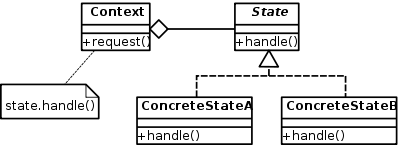
\includegraphics[scale=0.8]{state}
        \end{center}
        The three participants of this include:
        \begin{itemize}
            \item Context: Defines the status of the program that determine what state the object should be in
            \item State: The state of an object (interface for concrete states to inherit from)
            \item ConcreteState subclasses: The possible states of the object
        \end{itemize}

    \subsection{Proxy}

    \subsection{Chain of Responsibility}

    \subsection{Interpreter}

    \subsection{Mediator}

    \subsection{Memnto}

    \subsection{Visior}

\newpage

\section{Code}

    \subsection{Abstract Base Class (ABC)}
        \begin{lstlisting}
        // Application.java
        package edu.psu.cmpsc221;

        public class Application {
            public static void main(String[] args) {
                Honda car = new Civic();
                car.blowHorn();
                ((Civic) car).setCruiseControl();
            }
        }
        \end{lstlisting}

        \begin{lstlisting}
        //Civic.java
        package edu.psu.cmpsc221;

        public class Civic extends Honda {

            public Civic() {
                super(5000);
                odometer = 6;
            }

            @Override
            public void blowHorn() {
                System.out.println("Murp");
            }

            public void setCruiseControl() {
                System.out.println("Civic.setCruiseControl");
            }
        }
        \end{lstlisting}

        \begin{lstlisting}
        // Honda.java
        package edu.psu.cmpsc221;

        public abstract class Honda {
            public abstract void blowHorn();
            public Honda(int odometer) {
                this.odometer = odometer;
            }
            protected int odometer;
        }
        \end{lstlisting}

    \newpage

    \subsection{Arrays}
        \begin{lstlisting}
        // Appplication.java
        package edu.psu.cmpsc221;

        public class Application {
            public static void main(String[] args) {
                Parent me = new Parent();
                Parent someChild = new Child1();
                Parent someOtherChild = new Child2();

                me.parentStuff();
                someChild.parentStuff();
                someOtherChild.parentStuff();

                ((Child1) someChild).child1Stuff();
                ((Child2) someChild).child2Stuff();

                ((Child2) someOtherChild).child2Stuff();

            }
        }
        \end{lstlisting}

        \begin{lstlisting}
        // ArrayStuff.java
        package edu.psu.cmpsc221;

        public class ArrayStuff {
        //    public <R> R[] createArray(int length) {
        //        return new R[length];
        //    }

        public static void main(String[] args) {
            new ArrayStuff().run();
        }

        private void printArray(int[] array) {
            // Regular old boring for loop
            //        for (int index = 0; index < array.length; ++index) {
            //            System.out.println(array[index]);
            //        }

            // Enhanced for loop
            for (int element : array) {
                System.out.println(element);
            }
        }

            private void run() {
                int[] stuff = { 5, 6, 5, 6754, 234, 636, 22};

                printArray(stuff);
            }

        }
        \end{lstlisting}

        \begin{lstlisting}
        //Child1.java
        package edu.psu.cmpsc221;

        public class Child1 extends Parent {
            public void child1Stuff() {
                System.out.println("child1Stuff");
            }
        }
        \end{lstlisting}

        \begin{lstlisting}
        //Child2.java
        package edu.psu.cmpsc221;

        public class Child2 extends Parent {
            public void child2Stuff() {
                System.out.println("child2Stuff");
            }
        }
        \end{lstlisting}

        \begin{lstlisting}
        //Parent.java
        package edu.psu.cmpsc221;

        public class Parent {
            public void parentStuff() {
                System.out.println("parentStuff");
            }
        }
        \end{lstlisting}

    \newpage

    \subsection{Double Dispatch}
        \begin{lstlisting}
        // Application.java
        package edu.psu.cmpsc221;

        public class Application {
            public static void main(String[] args) {
                MyNumber adder = new MyFloat();
                MyNumber addend = new MyInteger();
                addend.add(adder);
            }
        }
        \end{lstlisting}

        \begin{lstlisting}
        // MyFloat.java
        package edu.psu.cmpsc221;

        public class MyFloat extends MyNumber {
            @Override
            public MyNumber add(MyNumber adder) {
                System.out.println("Unoptimized");
                return new MyFloat();
            }

            @Override
            protected MyNumber addToInteger(MyInteger adder) {
                System.out.println("Unoptimized");
                return new MyFloat();
            }
        }
        \end{lstlisting}

        \begin{lstlisting}
        // MyInteger.java
        package edu.psu.cmpsc221;

        public class MyInteger extends MyNumber {
            @Override
            public MyNumber add(MyNumber adder) {
                return adder.addToInteger(this);
            }

            @Override
            protected MyNumber addToInteger(MyInteger adder) {
                System.out.println("Optimized");
                return new MyInteger();
            }
        }
        \end{lstlisting}

        \begin{lstlisting}
        // MyNumber.java
        package edu.psu.cmpsc221;

        public abstract class MyNumber {
            public abstract MyNumber add(MyNumber adder);
            protected abstract MyNumber addToInteger(MyInteger adder);
        }
        \end{lstlisting}

    \newpage

    \subsection{Exception}
        \begin{lstlisting}
        //Application.java
        package edu.psu.cmpsc221;

        import java.io.BufferedWriter;
        import java.io.IOException;
        import java.nio.file.Files;
        import java.nio.file.Paths;

        public class Application {
            public static void main(String[] args) {
                new Application().run();
            }

            private void run() {
                try {
                    generateUncheckedException();
                } catch (IllegalArgumentException ex) {
                    ex.printStackTrace();
                    // Do something.  No-op
                    int a = 0;
                } catch (Exception ex) {
                    // I can handle this one differently
                }

                try {
                    generateCheckedException();
                } catch (Exception ex) {
                    // No-op
                }

                try {
                    generateMyException();
                } catch (MyException ex) {
                } catch (Exception ex) {
                } finally {
            //            file.close();
                }

                try (BufferedWriter bw = Files.newBufferedWriter(Paths.get("ripple.txt"))) {
                    bw.write("Hey, the king's back!");
                } catch (IOException e) {
                    e.printStackTrace();
                }

                System.out.println("I hope I get here");
            }

            private void generateUncheckedException() {
                throw new IllegalArgumentException("Hello, this is me");
            }

            private void generateCheckedException() throws Exception {
                throw new Exception("Hola, que pasa?");
            }

            private void generateMyException() throws MyException {
                throw new MyException("Hola, que pasa?");
            }

        } /* end Application */
        \end{lstlisting}

        \begin{lstlisting}
        //MyException.java
        package edu.psu.cmpsc221;

        public class MyException extends Exception {
            public MyException(String description) {
                super(description);
            }
        }
        \end{lstlisting}

    \newpage

    \subsection{Function}
        \begin{lstlisting}
        //Example.java
        package edu.psu.cmpsc221;

        public class Example {
            public static void main(String[] args) {
                Example example = new Example();
                example.executeFunction(new ComputeSuccessor(), 45);
                example.executeFunction(new ComputeSuccessor(), 2);
                example.executeFunction(new ComputeLength(), "Babe");
                example.executeFunction(new ComputeLength(), "Ripple");
                example.executeFunction(new ComputeDouble(), 45);
                example.executeFunction(new ComputeDouble(), 2);
            }

            private <R,D> void executeFunction(Function<R,D> function, D value) {
                System.out.println(function.apply(value));
            }

            private static class ComputeDouble implements Function<Integer, Integer> {
                @Override
                public Integer apply(Integer parameter) {
                    return parameter * 2;
                }
            }

            private static class ComputeSuccessor
                    implements Function<Integer, Integer> {
                @Override
                public Integer apply(Integer parameter) {
                    return parameter + 1;
                }
            }

            private static class ComputeLength implements Function<Integer, String> {
                @Override
                public Integer apply(String parameter) {
                    return parameter.length();
                }
            }
        }
        \end{lstlisting}

        \begin{lstlisting}
        //Function.java
        package edu.psu.cmpsc221;

        public interface Function<R, D> {
            public R apply(D parameter);
        }
        \end{lstlisting}

    \newpage

    \subsection{Interfaces}

        \begin{lstlisting}
        //Application.java
        package edu.psu.cmpsc221;

        import java.util.ArrayList;
        import java.util.Arrays;
        import java.util.List;

        public class Application {
            public static void main(String[] args) {
                int[] intArray = { 1, 2, 3, 4, 5 };

                int[] anotherIntArray = new int[5];
                anotherIntArray[0] = 1;
                anotherIntArray[1] = 2;
                anotherIntArray[2] = 3;
                anotherIntArray[3] = 4;
                anotherIntArray[4] = 5;

                List<Integer> anotherIntegerList =
                        Arrays.asList(1, 2, 3, 4, 5);
                anotherIntegerList.add(10);

                List<Integer> integerList = new ArrayList<>();
                integerList.add(1);
                integerList.add(2);
                integerList.add(3);
                integerList.add(4);
                integerList.add(5);

                List<String> stringList = new ArrayList<>();
                stringList.add("1");
                stringList.add("2");
                stringList.add("3");
                stringList.add("4");
                stringList.add("5");

            } /* end main */
        } /* end Application */
        \end{lstlisting}

        \begin{lstlisting}
        //Civic.java
        package edu.psu.cmpsc221;

        public class Civic implements HornyCar {
            @Override
            public void blowHorn() {
                System.out.println("Civic.blowHorn");
            }
        }
        \end{lstlisting}

        \begin{lstlisting}
        //HornyCar.java
        package edu.psu.cmpsc221;

        public interface HornyCar {
            public void blowHorn();
        } /* end HornyCar */
        \end{lstlisting}

    \newpage

    \subsection{Observer}
        \begin{lstlisting}
        //Application.java
        package edu.psu.cmpsc221;

        import javax.swing.*;
        import java.awt.event.ActionEvent;
        import java.awt.event.ActionListener;

        public class Application implements ActionListener {
            public static void main(String[] args) {
                new Application().run();
            } /* end main */

            @Override
            public void actionPerformed(ActionEvent e) {
                if (e.getSource().equals(t)) {
                    System.out.println("Wake up!  It's time to study!! (YAY!)");
                } /* end if */
            } /* end actionPerformed */

            private void run() {
                final int durationInMilliseconds = 1000;
                t = new Timer(durationInMilliseconds, this);
            //        t.setRepeats(false);
                t.start();

                try {
                    final long sleepInMilliseconds = 3000;
                    Thread.sleep(sleepInMilliseconds);
                } catch (InterruptedException e) {
                    e.printStackTrace();
                }

                System.out.println("I'm awake!!");
            }

            private Timer t;
        }
        \end{lstlisting}

    \newpage

    \subsection{Polymorphism}
        \begin{lstlisting}
        //Application.java
        package edu.psu.cmpsc221;

        public class Application {
            public static void main(String[] args) {
                Parent instance = new Child();
                //instance.inheritedMethod();
                Child.sInheritedMethod();
            } /* end main */
        } /* end Application */
        \end{lstlisting}

        \begin{lstlisting}
        //Application.java
        package edu.psu.cmpsc221;

        public class Application {
            public static void main(String[] args) {
                Parent instance = new Child();
                //instance.inheritedMethod();
                Child.sInheritedMethod();
            } /* end main */
        } /* end Application */
        \end{lstlisting}

        \begin{lstlisting}
        //Parent.java
        package edu.psu.cmpsc221;

        public class Parent {
            public static void sInheritedMethod() {
                sComputeSomething();
            } /* end sInheritedMethod */

            public void inheritedMethod() {
                computeSomething();
            } /* end inheritedMethod */

            public static void sComputeSomething() {
                System.out.println("In Parent");
            } /* end sComputeSomething */

            public void computeSomething() {
                System.out.println("In Parent");
            } /* end v */
        } /* end Parent */
        \end{lstlisting}

    \newpage

    \subsection{Singleton}
        \begin{lstlisting}
        //Singleton.java
        package edu.psu.cmpsc221;

        /**
        * This is a singleton design pattern example
        */
        public final class Singleton {
            private static Singleton instance;  // declaration
            //    private static int age = 18;        // definition

            /**
             * A constructor for the class
             */
            private Singleton() {
            } /* end Singleton */

            /**
             * Access the singleton instance of the class
             * @return The Singleton instance
             */
            public static Singleton getInstance() {
                if (null == instance) {
                    instance = new Singleton();
                } /* end if */

                return instance;
            } /* end getInstance */

            public static void main(String[] args) {
                if (Singleton.getInstance() == Singleton.getInstance()) {
                    System.out.println("yes");
                } else {
                    System.out.println("no");
                }
            }


        } /* end Singleton */
        \end{lstlisting}

    \newpage

    \subsection{RESTful}
        \begin{lstlisting}
        // Service.java

        package edu.psu.cmpsc221;

        import javax.ws.rs.GET;
        import javax.ws.rs.Path;
        import javax.ws.rs.Produces;
        import javax.ws.rs.core.MediaType;

        @Path("/helloWorld")
        public class Service {

            @GET
            @Produces(MediaType.TEXT_PLAIN)
            public String getString() {
                return "Hello, World!";
            }

            @GET
            @Produces(MediaType.TEXT_XML)
            public String getTextXml() {
                return "<?xml version=\"1.0\"?> <aTag>Hello, world!!</aTag>";
            }

        }

        ////////////////////////////////////////////////////////////////////////////

        // WSClient.java

        package edu.psu.cmpsc221;

        import java.net.URI;

        import javax.ws.rs.client.Client;
        import javax.ws.rs.client.ClientBuilder;
        import javax.ws.rs.client.WebTarget;
        import javax.ws.rs.core.MediaType;
        import javax.ws.rs.core.UriBuilder;

        import org.glassfish.jersey.client.ClientConfig;

        public class WSClient {

            // http://localhost:8080/rest/application.wadl
            // http://localhost:8080/rest/helloWorld

            public static void main(String[] args) {
                ClientConfig clientConfig = new ClientConfig();
                Client client = ClientBuilder.newClient(clientConfig);
                WebTarget target = client.target(getBaseURI());

                try {
                    String textPlain =
                            target.path("helloWorld")
                                    .request()
                                    .accept(MediaType.TEXT_PLAIN)
                                    .get(String.class);

                    System.out.println("For call to hello, requesting plain text, I got:");
                    System.out.println(textPlain);
                    System.out.println();
                } catch (javax.ws.rs.NotFoundException e) {
                    System.out.println("alas");
                }

                try {
                    String textXml =
                            target.path("helloWorld")
                                    .request()
                                    .accept(MediaType.TEXT_XML)
                                    .get(String.class);

                    System.out.println("For call to hello, requesting xml text, I got:");
                    System.out.println(textXml);
                    System.out.println();
                } catch (javax.ws.rs.NotFoundException e) {
                    System.out.println("alas");
                }
            }


            public static URI getBaseURI() {
                return UriBuilder.fromUri("http://localhost:8080/rest").build();
            }
        }

        ////////////////////////////////////////////////////////////////////////////

        // WSServer.java

        package edu.psu.cmpsc221;

        import org.glassfish.grizzly.http.server.HttpServer;
        import org.glassfish.jersey.grizzly2.httpserver.GrizzlyHttpServerFactory;
        import org.glassfish.jersey.server.ResourceConfig;

        import javax.ws.rs.core.UriBuilder;
        import java.net.URI;

        public class WSServer {
            public static void main(String[] args) {
                System.out.println("Starting grizzly server");
                    ResourceConfig resourceConfig = new ResourceConfig().packages("edu.psu.cmpsc221");
                    HttpServer httpServer = GrizzlyHttpServerFactory.createHttpServer(getBaseURI(), resourceConfig);
                    System.out.println("Started!");
            }

            public static URI getBaseURI() {
                return UriBuilder.fromUri("http://localhost:8080/rest").build();
            }
        }
        \end{lstlisting}


    \newpage

    \subsection{Adventure Game}
        Different design patterns at use in the game:
        \begin{itemize}
            \item Observer: Used in the GUI implementation of the game
            \item State: Changes availability of rooms or accessibility of objects depending on the state they are in. If player unlocks a door, state of room is changed and that room can now be entered.
            \item Strategy: We choose the implementation of inventory system. We choose the algorithm that determines how inventory can be accessed and changed.
            \item Singleton: getInstance to return instance. There is only one instance of the game.
        \end{itemize}

        \begin{itemize}
            \item Controller
            \begin{itemize}
                \item Application - Runs the instance of the game using the class Controller
                \item Controller - The interfacing aspect that interfaces between the model and view
                \item Parser - Enables and processes text commands such as “get, drop, go, etc”
            \end{itemize}
            \item Model
            \begin{itemize}
                \item Direction - The general direction of the game, parent of CompassDirection.
                \item CompassDirection - Compass direction is initialized here. Opposite directions method can be used.
                \item Model - The backend of the game that initializes the backend of the model.
                \item ModelObject - Gets the certain instance of Model. Singleton
                \item Item - Initializes all the item variables in the game
                \item InventorySystem - Creates an instance of the inventory system from ModelObject. Inventory is an arraylist that can be added or dropped.
                \item Room - Models rooms for our game.
                \item Player - The person you play as.
                \item MobileCharacter  - Movable Character that has a location.
                \item Map - Initializes the room of the game.
            \end{itemize}
            \item View
            \begin{itemize}
                \item Adventure - The instance that starts to run the whole game.
            \end{itemize}
        \end{itemize}

        \subsubsection{controller}
            \begin{lstlisting}
            // Application.java
            package edu.psu.cmpsc221.controller;

            public class Application {
                public static void main(String[] args) {
                    Controller controller = Controller.getInstance();
                    controller.run();
                } /* end main */
            } /* end Application */

            ////////////////////////////////////////////////////////////////////

            // Contoller.java
            package edu.psu.cmpsc221.controller;

            import edu.psu.cmpsc221.AdventureObject;
            import edu.psu.cmpsc221.model.Direction;
            import edu.psu.cmpsc221.model.Model;
            import edu.psu.cmpsc221.view.TextView;
            import edu.psu.cmpsc221.view.View;
            import edu.psu.cmpsc221.view.gui.GuiView;

            public class Controller extends AdventureObject {
                public Controller() {
                    initializeKeepPlaying();
                    initializeParser();
                    initializeView();
                } /* end Controller */

                public void drop(String itemName) {
                    getModel().drop(itemName);
                } /* end drop */

                public void get(String itemName) {
                    getModel().get(itemName);
                } /* end get */

                public String getCurrentRoomLookDescription() {
                    return getModel().getCurrentRoomLookDescription();
                } /* end getCurrentRoomLookDescription */

                public String getCurrentRoomLookExits() {
                    return getModel().getCurrentRoomLookExits();
                } /* end getCurrentRoomLookExits */

                public String getCurrentRoomLookItems() {
                    return getModel().getCurrentRoomLookItems();
                } /* end getCurrentRoomLookItems */

                public static Controller getInstance() {
                    return instance;
                } /* end getInstance */

                public String getInventoryString() {
                    return getModel().getInventoryString();
                } /* end getInventoryString*/

                private boolean getKeepPlaying() {
                    return keepPlaying;
                } /* end getKeepPlaying */

                private Model getModel() {
                    return Model.getInstance();
                } /* end getModel */

                private Parser getParser() {
                    return parser;
                } /* end getParser */

                private View getView() {
                    return view;
                } /* end View */

                public void go(Direction direction) {
                    getModel().go(direction);
                } /* end go */

                private void initializeKeepPlaying() {
                    setKeepPlaying(true);
                } /* end initializeKeepPlaying */

                private void initializeParser() {
                    parser = new Parser();
                } /* end initializeParser */

                private void initializeView() {
            //        view = new TextView();
                    view = new GuiView();
                } /* end initializeView */

                public void inventory() {
                    getView().inventory();
                } /* end inventory */

                private void parseCommand(String command) {
                    getParser().parseCommand(command);
                } /* end parseCommand */

                public void processCantGoDirection(String directionName) {
                    getView().processCantGoDirection(directionName);
                } /* end processCantGoDirection */

                public void processDropItemNotInInventory(String itemName) {
                    getView().processDropItemNotInInventory(itemName);
                } /* end processDropItemNotInInventory */

                public void processDropSuccessful(String itemName) {
                    getView().processDropSuccessful(itemName);
                } /* end processDropSuccessful */

                public void processGetItemNotInInventory(String itemName) {
                    getView().processGetItemNotInInventory(itemName);
                } /* end processGetItemNotInInventory */

                public void processGetSuccessful(String itemName) {
                    getView().processGetSuccessful(itemName);
                } /* end processGetSuccessful */

                public void processGoDirectionSuccessful() {
                    getView().look();
                } /* end processGoDirectionSuccessful */

                public void processInventoryFullException(String message) {
                    getView().processInventoryFullException(message);
                } /* end processInventoryFullException */

                public void processLook() {
                    getView().look();
                } /* end processLook */

                private void processNextUserCommand() {
                    String command = getView().getUserCommand();
                    parseCommand(command);
                } /* end processNextUserCommand */

                public void processQuitCommand() {
                    getView().processQuitCommand();
                    setKeepPlaying(false);
                } /* end processQuitCommand */

                public void processUnknownCommand(String command) {
                    getView().processUnknownCommand(command);
                } /* end processUnknownCommand */

                public void run() {
                    getView().look();

                    while (getKeepPlaying()) {
                        processNextUserCommand();
                    } /* end while */
                } /* end run */

                private void setKeepPlaying(boolean value) {
                    keepPlaying = value;
                } /* end setKeepPlaying*/

                private static Controller instance = new Controller();
                private boolean keepPlaying;
                private Parser parser;
                private View view;
            } /* end Controller */


            ////////////////////////////////////////////////////////////////////

            // Parser.java
            package edu.psu.cmpsc221.controller;

            import edu.psu.cmpsc221.AdventureObject;
            import edu.psu.cmpsc221.model.CompassDirection;
            import edu.psu.cmpsc221.model.Direction;

            public class Parser extends AdventureObject {
                public void parseCommand(String command) {
                    String[] commands = command.trim().toLowerCase().split(" ");

                    if (commands.length > 0) {
                        switch (commands[0]) {
                            case "drop" : processDrop(commands); break;

                            case "get" : processGet(commands); break;

                            case "go" : processGo(commands); break;
                            case CompassDirection.NORTH_NAME : processGo(CompassDirection.NORTH); break;
                            case CompassDirection.SOUTH_NAME : processGo(CompassDirection.SOUTH); break;
                            case CompassDirection.EAST_NAME : processGo(CompassDirection.EAST); break;
                            case CompassDirection.WEST_NAME : processGo(CompassDirection.WEST); break;

                            case "i" : // Fall through to the next entry
                            case "inventory" : processInventory(); break;

                            case "look" : getController().processLook(); break;

                            case "quit" : getController().processQuitCommand(); break;

                            default : getController().processUnknownCommand(command); break;
                        } /* end switch */
                    } /* end if */
                } /* end parseCommand */

                private void processDrop(String[] commands) {
                    getController().drop(commands.length > 1 ? commands[1] : "");
                } /* end processDrop */

                private void processGet(String[] commands) {
                    getController().get(commands.length > 1 ? commands[1] : "");
                } /* end processGet */

                private void processGo(Direction direction) {
                    getController().go(direction);
                } /* end processGo */

                private void processGo(String[] commands) {
                    boolean wasCommandsProcessed = false;

                    if (commands.length > 1) {
                        switch (commands[1]) {
                            case CompassDirection.NORTH_NAME : {
                                processGo(CompassDirection.NORTH);
                                wasCommandsProcessed = true;
                                break;
                            } /* end case */

                            case CompassDirection.SOUTH_NAME : {
                                processGo(CompassDirection.SOUTH);
                                wasCommandsProcessed = true;
                                break;
                            } /* end case */

                            case CompassDirection.EAST_NAME : {
                                processGo(CompassDirection.EAST);
                                wasCommandsProcessed = true;
                                break;
                            } /* end case */

                            case CompassDirection.WEST_NAME : {
                                processGo(CompassDirection.WEST);
                                wasCommandsProcessed = true;
                                break;
                            } /* end case */
                        } /* end switch */
                    } /* end if */

                    if (!wasCommandsProcessed) getController().processUnknownCommand(String.join(" ", commands));
                } /* end processGo */

                private void processInventory() {
                    getController().inventory();
                } /* end processInventory */

            } /* end Parser */



            \end{lstlisting}

        \newpage

        \subsubsection{excetions}
            \begin{lstlisting}
            // CantGoDirectionException.java
            package edu.psu.cmpsc221.exceptions;

            import edu.psu.cmpsc221.model.Direction;

            public class CantGoDirectionException extends Exception {
                public CantGoDirectionException(Direction direction) {
                    super(direction.getName());
                } /* end CantGoDirectionException */
            } /* end CantGoDirectionException */

            ////////////////////////////////////////////////////////////////////

            // InventryFullExcetion
            package edu.psu.cmpsc221.exceptions;

            import edu.psu.cmpsc221.model.Item;

            public class InventoryFullException extends Exception {
                public InventoryFullException(String message, Item item) {
                    super(message);
                    this.item = item;
                } /* end InventoryFullException */

                public Item getItem() {
                    return item;
                } /* end getItem */

                private Item item;
            } /* end InventoryFullException*/

            ////////////////////////////////////////////////////////////////////

            // ItemNotInInventory
            package edu.psu.cmpsc221.exceptions;

            import edu.psu.cmpsc221.model.Item;

            public class ItemNotInInventoryException extends Exception {
                public ItemNotInInventoryException(String itemName) {
                    super(itemName);
                } /* end ItemNotInInventoryException */

                public ItemNotInInventoryException(Item item) {
                    super(item.getName());
                } /* end ItemNotInInventoryException */
            } /* end ItemNotInInventoryException */
            \end{lstlisting}

        \newpage

        \subsubsection{model}
            \begin{lstlisting}
            // CompassDirection.java
            package edu.psu.cmpsc221.model;

            public class CompassDirection extends Direction {
                public static final String NORTH_NAME = "north";
                public static final String SOUTH_NAME = "south";
                public static final String EAST_NAME = "east";
                public static final String WEST_NAME = "west";

                public static final CompassDirection NORTH = new CompassDirection(NORTH_NAME);
                public static final CompassDirection SOUTH = new CompassDirection(SOUTH_NAME);
                public static final CompassDirection EAST = new CompassDirection(EAST_NAME);
                public static final CompassDirection WEST = new CompassDirection(WEST_NAME);

                static {
                    NORTH.setOppositeCompassDirection(SOUTH);
                    SOUTH.setOppositeCompassDirection(NORTH);
                    EAST.setOppositeCompassDirection(WEST);
                    WEST.setOppositeCompassDirection(EAST);
                } /* end static */

                public CompassDirection(String name) {
                    super(name);
                } /* end CompassDirection */

                CompassDirection getOppositeCompassDirection() {
                    return oppositeCompassDirection;
                } /* end setOppositeCompassDirection */

                private void setOppositeCompassDirection(CompassDirection compassDirection) {
                    this.oppositeCompassDirection = compassDirection;
                } /* end setOppositeCompassDirection */

                private CompassDirection oppositeCompassDirection;
            } /* end CompassDirection */

            ////////////////////////////////////////////////////////////////////

            // Direction.java

            package edu.psu.cmpsc221.model;

            /**
             * A general direction for teh [sic] game
             */
            public class Direction {
                public Direction(String name) {
                    this.name = name;
                } /* end Direction */

                public String getName() {
                    return name;
                } /* end getName */

                private String name;
            } /* end Direction */

            ////////////////////////////////////////////////////////////////////

            // InfiniteInventorySystem.java
            package edu.psu.cmpsc221.model;

            public class InfiniteInventorySystem extends InventorySystem {
                protected boolean canAddItem(Item item) {
                    return true;
                } /* end canAddItem */

                protected String getInventoryFullMessage() {
                    // This can't occur in this mode so just return an empty string
                    return "";
                } /* end getInventoryFullMessage */
            } /* end InfiniteInventorySystem */


            ////////////////////////////////////////////////////////////////////

            // InventorySystem.java
            package edu.psu.cmpsc221.model;

            import edu.psu.cmpsc221.exceptions.InventoryFullException;
            import edu.psu.cmpsc221.exceptions.ItemNotInInventoryException;

            import java.util.ArrayList;
            import java.util.List;
            import java.util.stream.Collectors;

            public abstract class InventorySystem extends ModelObject {
                protected InventorySystem() {
                    list = new ArrayList<>();
                } /* end InventorySystem */

                void add(Item item) throws InventoryFullException {
                    if (canAddItem(item)) {
                        list.add(item);
                    } else {
                        throw new InventoryFullException(getInventoryFullMessage(), item);
                    } /* end if */
                } /* end add */

                protected abstract boolean canAddItem(Item item);

                void dropAll() {
                    while (!list.isEmpty()) {
                        try {
                            drop(list.get(0));
                        } catch (ItemNotInInventoryException e) {
                            // No-op.  This can't occur
                        } /* end try */
                    } /* end while */
                } /* end dropAll */

                void drop(Item item) throws ItemNotInInventoryException {
                    remove(item);
                    getModel().addToCurrentRoomInventory(item);
                } /* end drop */

                protected abstract String getInventoryFullMessage();

                String getInventoryString() {
                    String inventoryString =
                       (list.isEmpty() ?
                        "You aren't carrying anything." :
                        "You are carrying: " + list.stream().map(Item::getName).collect(Collectors.joining(", ")));

                    return inventoryString;
                } /* end getInventoryString */

                String getLookItems() {
                    String lookItems =
                       (list.isEmpty() ?
                        "" :
                        list.stream().map(Item::getLookDescription).collect(Collectors.joining(System.lineSeparator())) + System.lineSeparator());

                    return lookItems;
                } /* end getLookItems */

                protected void remove(Item item) throws ItemNotInInventoryException {
                    if (!list.remove(item)) throw new ItemNotInInventoryException(item);
                } /* end remove */

                Item removeItemNamed(String itemName) throws ItemNotInInventoryException {
                    // Can use lambdas, but we'll do it manually
                    for (Item item : list) {
                        if (item.getName().equals(itemName)) {
                            list.remove(item);
                            return item;
                        } /* end if */
                    } /* end for */

                    throw new ItemNotInInventoryException(itemName);
                } /* end removeItemNamed */

                List<Item> list;
            } /* end InventorySystem */

            ////////////////////////////////////////////////////////////////////

            // Item.java

            package edu.psu.cmpsc221.model;

            public class Item {
                public Item(String name, String lookDescription) {
                    this.lookDescription = lookDescription;
                    this.name = name;
                } /* end Item */

                public String getLookDescription() {
                    return lookDescription;
                } /* end getLookDescription */

                public String getName() {
                    return name;
                } /* end getName */

                private String lookDescription;
                private String name;
            } /* end Item */

            ////////////////////////////////////////////////////////////////////

            // Map.java
            package edu.psu.cmpsc221.model;

            public class Map {
               public Map() {
                  thomas101 =
                     new Room("You are seated in 101 Thomas Building.  It is brightly lit and is the site of your favourite class OF ALL TIME.  Evaaaar.",
                             "101Thomas");
                  thomasHallway = new Room("You are in the main hallway on the first floor of Thomas Building.", "ThomasFirstHallway");
                  thomasEastExit = new Room("You are standing outside Thomas Building along Pollock Road", "thomasEastExit");
                  mcElwainCourtyard = new Room("You are in McElwain's courtyard, a peaceful beautiful setting reminiscent of earlier times.", "(mcElwain");

                  thomas101.addCompassExit(CompassDirection.SOUTH, thomasHallway);
                  thomasHallway.addCompassExit(CompassDirection.EAST, thomasEastExit);
                  thomasEastExit.addCompassExit(CompassDirection.EAST, mcElwainCourtyard);

                  thomas101.addToInventory(new Item("ball", "A fully inflated beach ball lies nearby."));
                  thomas101.addToInventory(new Item("pen", "A totally dried up dry-write pen is discarded here."));
                  thomas101.addToInventory(new Item("laptop", "There is a laptop here."));
                  thomas101.addToInventory(new Item("books", "A large pile of computer science books sits on a desk."));
                  thomas101.addToInventory(new Item("bookbag", "A rather heavy bookbag sits unattended in the room."));
                  thomas101.addToInventory(new Item("homework", "A thick pile of unclaimed homework sits on the front table."));
               } /* end Map */

               public Room getInitialPlayerRoom() {
                  return thomas101;
               } /* end getInitialPlayerRoom */

               private Room thomas101;
               private Room thomasHallway;
               private Room thomasEastExit;
               private Room mcElwainCourtyard;
            } /* end Map */

            ////////////////////////////////////////////////////////////////////

            // MobileCharacter.java

            package edu.psu.cmpsc221.model;

            import edu.psu.cmpsc221.exceptions.CantGoDirectionException;

            public abstract class MobileCharacter extends ModelObject {
                protected MobileCharacter() {
                    // Subclasses must independently initialize their current room.  We
                    // can't drive that here because we only have a proto-object!
                } /* end MobileCharacter */

                protected Room getCurrentRoom() {
                    return currentRoom;
                } /* end getCurrentRoom */

                public String getCurrentRoomLookDescription() {
                    return getCurrentRoom().getLookDescription();
                } /* end getCurrentRoomLookDescription */

                public String getCurrentRoomLookExits() {
                    return getCurrentRoom().getLookExits();
                } /* end getCurrentRoomLookExits */

                public String getCurrentRoomLookItems() {
                    return getCurrentRoom().getLookItems();
                } /* end getCurrentRoomLookItems*/

                protected void go(Direction direction) throws CantGoDirectionException {
                    setCurrentRoom(getCurrentRoom().go(direction));
                } /* end go */

                protected abstract void initializeCurrentRoom();

                protected void setCurrentRoom(Room room) {
                    currentRoom = room;
                } /* end setCurrentRoom */

                private Room currentRoom;
            } /* end MobileCharacter */

            ////////////////////////////////////////////////////////////////////

            // Model.java

            package edu.psu.cmpsc221.model;

            public class Model {
                private static Model instance;

                static {
                    instance = new Model();
                    // The model, itself, as well as both the map and the player must exist
                    // before they can be properly initialized.
                    instance.initialize();
                } /* end static */

                protected Model() {
                    map = new Map();
                    player = new Player();
                } /* end Model */

                void addToCurrentRoomInventory(Item item) {
                    getPlayer().addToCurrentRoomInventory(item);
                } /* end addToCurrentRoomInventory */

                public void drop(String itemName) {
                    getPlayer().drop(itemName);
                } /* end drop */

                public void get(String itemName) {
                    getPlayer().get(itemName);
                } /* end get */

                public String getCurrentRoomLookDescription() {
                    return getPlayer().getCurrentRoomLookDescription();
                } /* end getCurrentRoomLookDescription */

                public String getCurrentRoomLookExits() {
                    return getPlayer().getCurrentRoomLookExits();
                } /* end getCurrentRoomLookExits */

                public String getCurrentRoomLookItems() {
                    return getPlayer().getCurrentRoomLookItems();
                } /* end getCurrentRoomLookItems*/

                public static Model getInstance() {
                    return instance;
                } /* end getInstance */

                public String getInventoryString() {
                    return getPlayer().getInventoryString();
                } /* end getInventoryString */

                public Room getInitialPlayerRoom() {
                    return getMap().getInitialPlayerRoom();
                } /* end getInitialPlayerRoom */

                Map getMap() {
                    return map;
                } /* end getMap */

                Player getPlayer() {
                    return player;
                } /* end getPlayer */

                public void go(Direction direction) {
                    getPlayer().go(direction);
                } /* end go */

                private void initialize() {
                    getPlayer().initialize();
                } /* end initialize */

                private Map map;
                private Player player;
            } /* end Model */

            ////////////////////////////////////////////////////////////////////

            // ModelObject.java

            package edu.psu.cmpsc221.model;

            import edu.psu.cmpsc221.AdventureObject;

            public class ModelObject extends AdventureObject {
                protected Model getModel() {
                    return Model.getInstance();
                } /* end getModel */
            } /* end ModelObject */

            ////////////////////////////////////////////////////////////////////

            // Player.java

            package edu.psu.cmpsc221.model;

            import edu.psu.cmpsc221.exceptions.CantGoDirectionException;
            import edu.psu.cmpsc221.exceptions.InventoryFullException;
            import edu.psu.cmpsc221.exceptions.ItemNotInInventoryException;

            public class Player extends MobileCharacter {
                public Player() {
                    // We cannot initialize the current room yet.  We only have a proto-object!
                    inventorySystem = new ZeroInventorySystem();
                } /* end Player */

                void addToCurrentRoomInventory(Item item) {
                    getCurrentRoom().addToInventory(item);
                } /* end addToCurrentRoomInventory */

                private void addToInventory(Item item) throws InventoryFullException {
                    inventorySystem.add(item);
                } /* end addToInventory */

                public void drop(String itemName) {
                    try {
                        Item item = removeFromInventory(itemName);
                        addToCurrentRoomInventory(item);
                        getController().processDropSuccessful(itemName);
                    } catch (ItemNotInInventoryException e) {
                        getController().processDropItemNotInInventory(e.getMessage());
                    } /* end catch */
                } /* end drop */

                public void get(String itemName) {
                    try {
                        Item item = removeFromCurrentRoomInventory(itemName);
                        addToInventory(item);
                        getController().processGetSuccessful(itemName);
                    } catch (ItemNotInInventoryException e) {
                        getController().processGetItemNotInInventory(itemName);
                    } catch (InventoryFullException e) {
                        addToCurrentRoomInventory(e.getItem());
                        getController().processInventoryFullException(e.getMessage());
                    } /* end try */
                } /* end get */

                String getInventoryString() {
                    return inventorySystem.getInventoryString();
                } /* end getInventoryString */

                public void go(Direction direction) {
                    try {
                        super.go(direction);
                        getController().processGoDirectionSuccessful();
                    } catch (CantGoDirectionException e) {
                        getController().processCantGoDirection(e.getMessage());
                    } /* end try */
                } /* end go */

                void initialize() {
                    initializeCurrentRoom();
                } /* end initialize */

                protected void initializeCurrentRoom() {
                    setCurrentRoom(getModel().getInitialPlayerRoom());
                } /* end initializeCurrentRoom */

                private Item removeFromCurrentRoomInventory(String itemName) throws ItemNotInInventoryException {
                    return getCurrentRoom().removeFromInventory(itemName);
                } /* end removeFromCurrentRoomInventory */

                private Item removeFromInventory(String itemName) throws ItemNotInInventoryException {
                    return inventorySystem.removeItemNamed(itemName);
                } /* end removeFromInventory */

                private InventorySystem inventorySystem;
            } /* end Player */

            ////////////////////////////////////////////////////////////////////

            // Room.java

            package edu.psu.cmpsc221.model;

            import edu.psu.cmpsc221.exceptions.CantGoDirectionException;
            import edu.psu.cmpsc221.exceptions.InventoryFullException;
            import edu.psu.cmpsc221.exceptions.ItemNotInInventoryException;

            import java.util.HashMap;
            import java.util.Map;
            import java.util.stream.Collectors;

            /**
             * This class models rooms in our adventure game
             */
            public class Room {

                Room(String lookDescription, String name) {
                    this.exits = new HashMap<>();
                    this.inventorySystem = new InfiniteInventorySystem();
                    this.lookDescription = lookDescription;
                    this.name = name;
                } /* end Room */

                void addCompassExit(CompassDirection compassDirection, Room toRoom) {
                    addExit(compassDirection, toRoom);
                    toRoom.addExit(compassDirection.getOppositeCompassDirection(), this);
                } /* end addCompassExit */

                void addExit(Direction direction, Room toRoom) {
                    exits.put(direction, toRoom);
                } /* end addExit */

                void addToInventory(Item item) {
                    try {
                        inventorySystem.add(item);
                    } catch (InventoryFullException e) {
                        // No-op.  This won't occur.
                    } /* end try */
                } /* end addToInventory*/

                private Room getExitForDirection(Direction direction) throws CantGoDirectionException {
                    Room candidateRoom = exits.get(direction);
                    if (null == candidateRoom) throw new CantGoDirectionException(direction);
                    return candidateRoom;
                } /* end getExitForDirection */

                public String getLookDescription() {
                    return lookDescription;
                } /* end getLookDescription */

                public String getLookExits() {
                    String lookExits = "Obvious exits are to the ";
                    String exitsAsString =
                       exits.keySet().stream().map(Direction::getName).collect(Collectors.joining(", "));
                    lookExits += exitsAsString; // lookExits = lookExits + exitsAsString;
                    return lookExits;
                } /* end getLookExits */

                public String getLookItems() {
                    return inventorySystem.getLookItems();
                } /* end getLookItems */

                public Room go(Direction direction) throws CantGoDirectionException {
                    return getExitForDirection(direction);
                } /* end go */

                Item removeFromInventory(String itemName) throws ItemNotInInventoryException {
                    return inventorySystem.removeItemNamed(itemName);
                } /* end removeFromInventory */

                private Map<Direction, Room> exits;
                private InventorySystem inventorySystem;
                private String lookDescription;
                private String name;
            } /* end Room */


            ////////////////////////////////////////////////////////////////////

            // ZeroInventorySystem.java

            package edu.psu.cmpsc221.model;

            public class ZeroInventorySystem extends InventorySystem {
                protected boolean canAddItem(Item item) {
                    return false;
                } /* end canAddItem */

                protected String getInventoryFullMessage() {
                    return "It falls through my pockets and back onto the floor.";
                } /* end getInventoryFullMessage */
            } /* end ZeroInventorySystem */
            \end{lstlisting}

        \newpage

        \begin{lstlisting}
        // AdventureObject.java
        package edu.psu.cmpsc221;

        import edu.psu.cmpsc221.controller.Controller;

        public class AdventureObject {
            protected Controller getController() {
                return Controller.getInstance();
            } /* end getController */
        } /* end AdventureObject */
        \end{lstlisting}


\end{document}
